%!Tex Root = ../Tutorat1.tex
% ./Packete.tex
% ./Design.tex
% ./Deklarationen.tex

\section{Exercise 1 - Memory Addresses}

\begin{frame}[fragile]{Exercise 1 - Memory Addresses}{Exercise 1.1}
  \begin{solution}
    \begin{columns}
      \begin{column}{0.2\textwidth}
        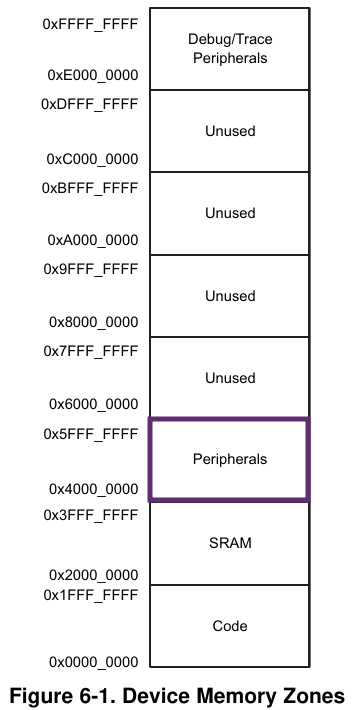
\includegraphics[height=0.5\paperheight]{./figures/peripherals.png}
      \end{column}
      \begin{column}{0.8\textwidth}
        \begin{itemize}
          \item $0x5FFF\_FFFF - 0x4000\_0000 + 1 = 0x2000\_0000$
          \item $0x2000\_0000 = 2 \cdot 16^7 = 2 \cdot {(2^4)}^7 = 2 \cdot 2^{4\cdot 7} = 2^{1+28} = 2^{29}$
        \end{itemize}
      \end{column}
    \end{columns}
  \end{solution}
\end{frame}

\begin{frame}{Exercise 1 - Memory Addresses}{Exercise 1.1}
  \begin{solution}
    \begin{columns}
      \begin{column}{0.4\textwidth}
        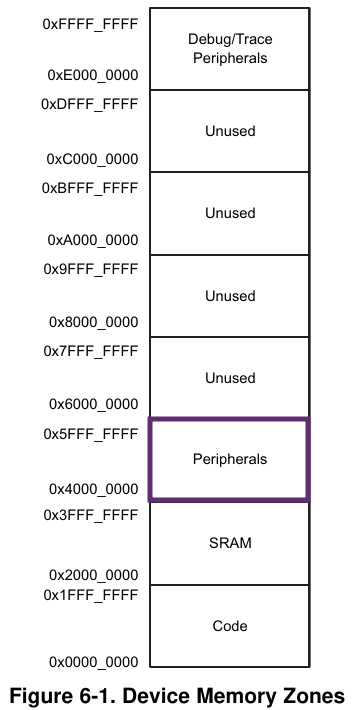
\includegraphics[height=0.5\paperheight]{./figures/peripherals.png}
        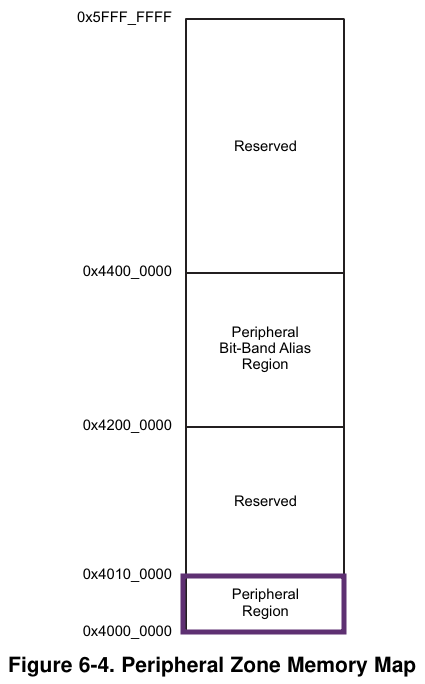
\includegraphics[height=0.5\paperheight]{./figures/peripherals_region.png}
      \end{column}
      \begin{column}{0.6\textwidth}
        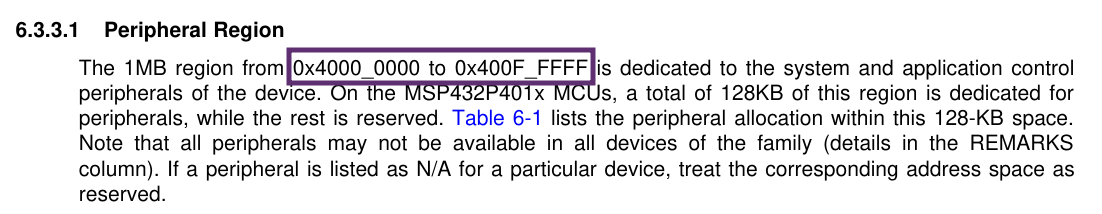
\includegraphics[width=0.5\paperwidth]{./figures/system_and_application_control_peripherals.png}
        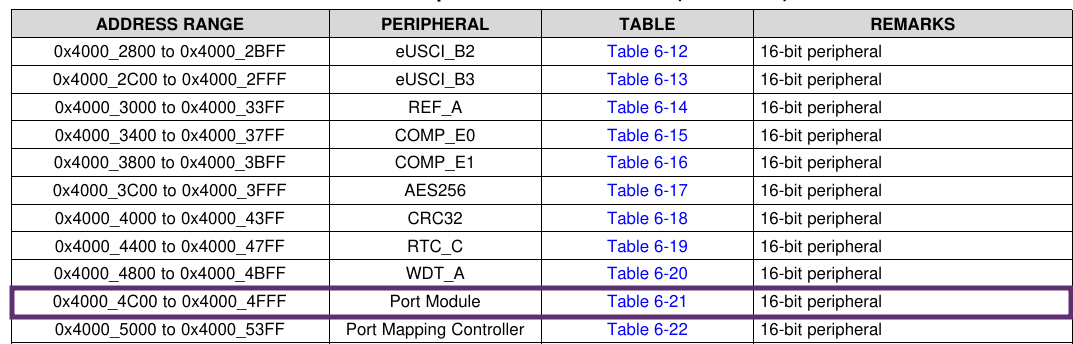
\includegraphics[width=0.5\paperwidth]{./figures/port_module.png}
      \end{column}
    \end{columns}
    \begin{itemize}
      \item $0x4000\_4FFF - 0x4000\_4C00 + 1 = 0x0400$
      \item $0x0400 = 4 \cdot 16^2 = 2^2 \cdot {(2^4)}^2 = 2^2 \cdot 2^{(4\cdot 2)} = 2^{2+8} = 2^{10}$
    \end{itemize}
  \end{solution}
\end{frame}

\begin{frame}{Exercise 1 - Memory Addresses}{Exercise 1.1}
  \begin{solution}
    \begin{columns}
      \begin{column}{0.4\paperwidth}
        \centering
        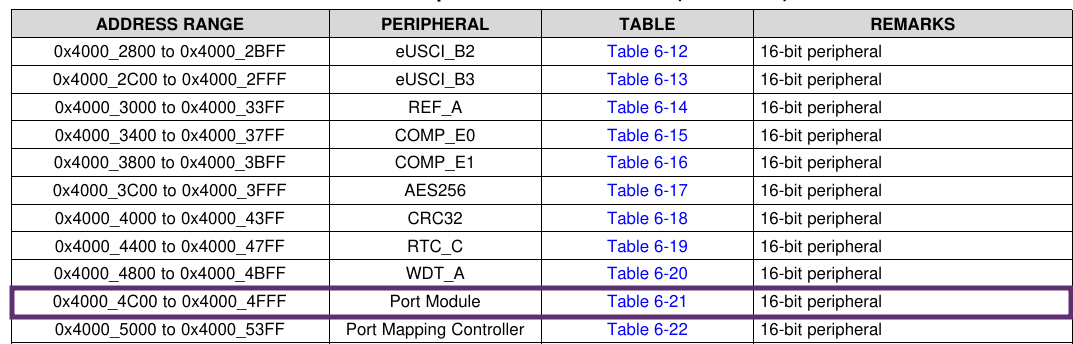
\includegraphics[width=0.3\paperwidth]{./figures/port_module.png}
        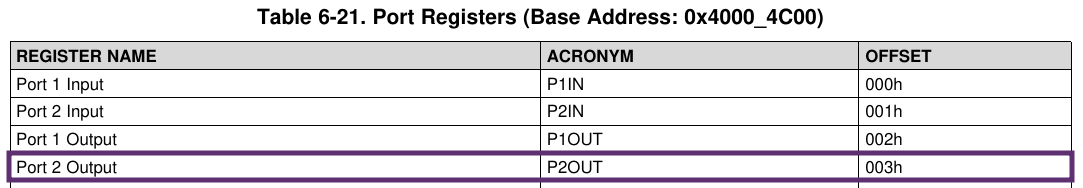
\includegraphics[width=0.3\paperwidth]{./figures/port2.png}
      \end{column}
      \begin{column}{0.6\paperwidth}
        \begin{itemize}
          \item $0x4000\_4C00 + 0x0003 = 0x4000\_4C03$
        \end{itemize}
      \end{column}
    \end{columns}
  \end{solution}
\end{frame}
